\begin{equation}
    \begin{aligned}
        \begin{gathered}
            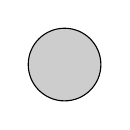
\begin{tikzpicture}[x=0.75pt,y=0.75pt,yscale=-0.7,xscale=0.7]
                %uncomment if require: \path (0,300); %set diagram left start at 0, and has height of 300
                
                %Shape: Circle [id:dp25295678135186517] 
                \draw  [fill={rgb, 255:red, 155; green, 155; blue, 155 }  ,fill opacity=0.5 ] (114,120) .. controls (114,106.19) and (125.19,95) .. (139,95) .. controls (152.81,95) and (164,106.19) .. (164,120) .. controls (164,133.81) and (152.81,145) .. (139,145) .. controls (125.19,145) and (114,133.81) .. (114,120) -- cycle ;
                \end{tikzpicture}            
        \end{gathered} \quad &= \quad \begin{gathered}
            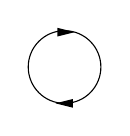
\begin{tikzpicture}[x=0.75pt,y=0.75pt,yscale=-0.7,xscale=0.7]
                %uncomment if require: \path (0,300); %set diagram left start at 0, and has height of 300
                
                %Shape: Circle [id:dp25295678135186517] 
                \draw  [fill={rgb, 255:red, 255; green, 255; blue, 255 }  ,fill opacity=1 ] (114,120) .. controls (114,106.19) and (125.19,95) .. (139,95) .. controls (152.81,95) and (164,106.19) .. (164,120) .. controls (164,133.81) and (152.81,145) .. (139,145) .. controls (125.19,145) and (114,133.81) .. (114,120) -- cycle ;
                %Straight Lines [id:da3302260003559434] 
                \draw    (146,96) ;
                \draw [shift={(146,96)}, rotate = 180] [fill={rgb, 255:red, 0; green, 0; blue, 0 }  ][line width=0.08]  [draw opacity=0] (12,-3) -- (0,0) -- (12,3) -- cycle    ;
                %Straight Lines [id:da744246828754719] 
                \draw    (140,145) -- (134.71,145) ;
                \draw [shift={(132.71,145)}, rotate = 360] [fill={rgb, 255:red, 0; green, 0; blue, 0 }  ][line width=0.08]  [draw opacity=0] (12,-3) -- (0,0) -- (12,3) -- cycle    ;
                \end{tikzpicture}        
        \end{gathered} \quad + \quad \begin{gathered}
            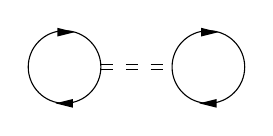
\begin{tikzpicture}[x=0.75pt,y=0.75pt,yscale=-0.7,xscale=0.7]
                %uncomment if require: \path (0,300); %set diagram left start at 0, and has height of 300
                
                %Shape: Circle [id:dp25295678135186517] 
                \draw  [fill={rgb, 255:red, 255; green, 255; blue, 255 }  ,fill opacity=1 ] (114,120) .. controls (114,106.19) and (125.19,95) .. (139,95) .. controls (152.81,95) and (164,106.19) .. (164,120) .. controls (164,133.81) and (152.81,145) .. (139,145) .. controls (125.19,145) and (114,133.81) .. (114,120) -- cycle ;
                %Straight Lines [id:da3302260003559434] 
                \draw    (146,96) ;
                \draw [shift={(146,96)}, rotate = 180] [fill={rgb, 255:red, 0; green, 0; blue, 0 }  ][line width=0.08]  [draw opacity=0] (12,-3) -- (0,0) -- (12,3) -- cycle    ;
                %Straight Lines [id:da744246828754719] 
                \draw    (140,145) -- (134.71,145) ;
                \draw [shift={(132.71,145)}, rotate = 360] [fill={rgb, 255:red, 0; green, 0; blue, 0 }  ][line width=0.08]  [draw opacity=0] (12,-3) -- (0,0) -- (12,3) -- cycle    ;
                %Shape: Circle [id:dp04752317906905801] 
                \draw  [fill={rgb, 255:red, 255; green, 255; blue, 255 }  ,fill opacity=1 ] (213,120) .. controls (213,106.19) and (224.19,95) .. (238,95) .. controls (251.81,95) and (263,106.19) .. (263,120) .. controls (263,133.81) and (251.81,145) .. (238,145) .. controls (224.19,145) and (213,133.81) .. (213,120) -- cycle ;
                %Straight Lines [id:da4128638497812116] 
                \draw    (245,96) ;
                \draw [shift={(245,96)}, rotate = 180] [fill={rgb, 255:red, 0; green, 0; blue, 0 }  ][line width=0.08]  [draw opacity=0] (12,-3) -- (0,0) -- (12,3) -- cycle    ;
                %Straight Lines [id:da9001038688985299] 
                \draw    (239,145) -- (233.71,145) ;
                \draw [shift={(231.71,145)}, rotate = 360] [fill={rgb, 255:red, 0; green, 0; blue, 0 }  ][line width=0.08]  [draw opacity=0] (12,-3) -- (0,0) -- (12,3) -- cycle    ;
                %Straight Lines [id:da6548078805333186] 
                \draw  [dash pattern={on 4.5pt off 4.5pt}]  (164,118.5) -- (213,118.5)(164,121.5) -- (213,121.5) ;
                \end{tikzpicture}            
        \end{gathered} \\
        &= \ii M_{\vb*{q}} \ii \Pi^0_q \ii M_{- \vb*{q}} + \ii M_{\vb*{q}} \ii \Pi^0_q (- \ii V^\text{eff}_q) \ii \Pi^0_q \ii M_{- \vb*{q}} \\ 
        &= - \ii \Pi^0_q \abs*{M_{\vb*{q}}}^2 - \ii \abs*{M_{\vb*{q}}}^2 (\Pi^0_q)^2 V^\text{eff}_q,
    \end{aligned}
\end{equation}